\documentclass[times, 10pt,twocolumn]{article} 
\usepackage{latex8}
\usepackage{times}
\usepackage{amsmath}
\usepackage{amsthm}
\usepackage{graphicx}
\usepackage{url}
%\usepackage[utf8x]{inputenc}
%\usepackage[brazil]{babel} 
%\usepackage[latin1]{inputenc}
%\usepackage[T1]{fontenc}
\usepackage{color}
\usepackage{subfig}

\newtheorem{theorem}{Theorem}[section]

\newcommand{\comentario}[1]{}
\newcommand{\superscript}[1]{\ensuremath{^{\textrm{#1}}}}
\newcounter{notecounter}
\newcommand{\nota}[1]{\addtocounter{notecounter}{1}{\textcolor{red}{[nota
      \arabic{notecounter}: #1]}}}

\newcommand{\gnota}[1]{
  \addtocounter{notecounter}{1}
  \vspace{.5cm}
  \framebox{
    \begin{minipage}{0.95\linewidth}
      \textbf{nota \arabic{notecounter}:} #1
    \end{minipage}
  }\vspace{.5cm}}

\newcommand{\simul}{\textbf{RTSimul}} % Que criatividade. Mudar esse
% nome depois, urgente

\author{Alexandre Passos, George Lima, Jos\'e Augusto Matos Santos}
%\address{Universidade Federal da Bahia}
\title{On the Use of Hard and Soft Reservation Schemes in \\ Constant Bandwidth Servers}

\begin{document}

\graphicspath{{figs/}{data/}}

\maketitle

\begin{abstract}

  When scheduling soft real-time tasks it is usually a good idea to
  reserve fractions of the total bandwidth to each task (or task
  group). This reservation might be either \textbf{hard}, when under
  no circumstances a task might use some extra bandwidth, or
  \textbf{soft}, if there are some situations when it is allowed to do
  so. Usually, specially in the context of on-line adaptative systems,
  hard reservation is perceived to be more predictable, stricter and
  allowing faster adaptation. In this paper we argue that, perhaps
  surprisingly, allowing tasks to use some idle bandwidth shouldn't
  hurt their performance and reliability. To clarify our arguments we
  present the results of a few experiments performed on real-life and
  syntetic data sets using hard and soft variations of CBS, a commonly
  used reservation-based server.
  
\end{abstract}

\Section{Introduction}
\label{sec:introduction}

\textbf{Context}.  Real-time systems once structured as a set of
simple periodic hard tasks \cite{liu.ea73:scheduling} have become
reasonably complex. Nowadays such systems are often composed of hard
and soft real-time tasks, which can be both periodic and non-periodic.
Usual requirements of these modern real-time systems include not only
predictability but also responsiveness and adaptiveness. In this
context, reservation-based scheduling, \textbf{RBS} for short, has
successfully been applied to support such requirements
\cite{abeni.ea04:resource,mercer.ea94:processor,rajkumar.ea98:resource,sprunt.ea89:aperiodic,steffens.ea03:resource}.

RBS techniques are usually implemented by scheduling servers. A server
is a virtual task responsible for scheduling application tasks
assigned to it.  Each server $S_i$ can be defined by a processor
reservation tuple, $(Q_i,T_i)$, where $Q_i$ is called the server
capacity and $T_i$ the server period.  If a task (or group of tasks)
$\tau$ is assigned to a server $S_i$, $\tau$ has the right to use
$Q_i$ processor time within $T_i$ time units. Hence, servers can then
be scheduled as if they were simple periodic tasks.

On top of its conceptual simplicity, RBS has several interesting
properties \cite{steffens.ea03:resource}. From the scheduling
viewpoint it is worthing mentioning that: (a) RBS is a means of
ensuring temporal isolation since task execution can be controlled
within its reservation envelop
\cite{abeni.ea04:resource,mercer.ea94:processor,sprunt.ea89:aperiodic,spuri.ea96:scheduling};
(b) it is possible to implement hierarchical scheduling when a group
of tasks share the same server
\cite{davis.ea05:hierarchical,davis.ea08:investigation}; (c) it can be
used to improve flexibility, responsiveness and adaptiveness at the
scheduler level.  Such characteristics have motivated considerable
research in the area
\cite{abeni.ea99:adaptive,caccamo.ea00:capacity,caccamo.ea05:efficient,oliveira.ea08:dynamic,oliveira.ea09:dynamic,lin.ea05:improving}.
In this paper we aim at better characterizing the performance of two
reservation schemes commonly implemented in real-time systems.

\textbf{Focus}.  A reservation scheme is \textbf{hard} if a server
$S_i = (Q_i,T_i)$ cannot be scheduled run for more than $Q_i$ time
units within any time interval of $T_i$ units even if there is idle
processor time available. On the other hand, a \textbf{soft} scheme
allows $S_i$ to execute beyond its reservation as long as system
schedulability is not compromised. Often the decision of implementing
one of these schemes arises. One of the widely known implementations
of soft RBS scheme in EDF scheduled systems is the Constant Bandwidth
Servers (\textbf{CBS}) \cite{abeni.ea04:resource}.  Due to the number
of other scheduling mechanisms based on CBS
\cite{abeni.ea05:qos,caccamo.ea00:capacity,caccamo.ea05:efficient,lipari.ea00:greedy},
we chose it as a case study in this paper.

According to the CBS rules, a constant bandwidth $u_i = Q_i/T_i$ is
allocated to each server $S_i = (Q_i,T_i)$, where $Q_i$ is called
hereafter the maximum server budget. The budget of each server $S_i$
is consumed as its jobs are executed. To guarantee that the server
obeys its utilization limit, the deadline of $S_i$ is postponed by
$T_i$ every time its budget is depleted.  Its full budget $Q_i$ is
also restored when its deadline is updated.  Deadline postponements
make it possible to implement the soft reservation scheme but brings
about a potential side effect: an overloaded server may have its
deadline postponed too often making its relative priority too low.
This problem may be avoided by implementing a hard reservation version
of CBS \cite{buttazzo05:soft}, which waits until the current server
deadline to recharge the server budget.  Nonetheless, it is still to
be checked whether soft or hard CBS performs better.

\textbf{Related work}. There is extensive research on comparing RBS
techniques.  Some of them have been on fixed-priority scheduling
\cite{bernat.ea99:new,bernat.ea02:multiple,davis.ea05:hierarchical,davis.ea95:dual}.
In the field of dynamic scheduling, CBS has been compared to several
other approaches \cite{spuri.ea96:scheduling}.  Techniques to
reclaiming spare capacity of CBS have also been reported, bringing in
comparative studies on their performance
\cite{caccamo.ea00:capacity,lin.ea05:improving}. To the best of our
knowledge these comparative studies have considered only the soft
version of CBS, though.  The work by Rajkumar et
al. \cite{rajkumar.ea01:resource} illustrates the use of hard and soft
versions of a fixed-priority RBS using a very simple task set.

\SubSection{Contributions of this paper}
\label{sec:contr-this-paper}

We report a comprehensive comparative study on the performance of
CBS. The reported evaluation puts into perspective the perceived
characteristics of its hard and soft reservation schemes.  By
benchmarking these two CBS versions in a simulation environment, they
are systematically compared against each other.  Since the use of CBS
has extensively been reported and one usually chooses arbitrarily
between these two versions
(e.g. \cite{abeni.ea99:adaptive,abeni.ea05:qos}), the results reported
here can better subsidize their implementation decisions.  The
reported study was carried out making use of the real-time scheduling
simulator \simul{}, implemented in Pyton. Although there are other
simulation tools \nota{citar simTools}, implementing this simulator
ourselves allowed us to easily tune it to our specific requirements.

\SubSection{Structure of this paper}
\label{sec:structure-this-paper}

Section \ref{sec:simul-envir} describes the system model and the
simulation environment.  In order to give a wide picture of the
simulated scheduling mechanisms, we conducted the evaluation taken
into consideration several metrics and different simulation scenarios,
which are presented in Section \ref{sec:metrics}. Results from the
simulation are discussed in Section \ref{sec:simulation-results} while
in Section \ref{sec:conclusion} our final comments are given.

\Section{Simulation Environment}
\label{sec:simul-envir}

To perform the experiments presented in this paper we implemented
\simul{}, a simple python-based simulator for real-time scheduling
algorithms. Its source code, the data files used in this paper and
instructions to reproduce our results are available in
\url{http://github.com/jamsjr/hard-versus-soft/tree/master}. \simul{}
implements a basic EDF scheduler and, on top of it, runs both hard
real-time periodic tasks and bandwidth sharing servers. These servers
can be either traditional CBS servers \cite{abeni.ea98:integrating} or
a hard reservation adaptation of the CBS algorithm, as described in
\cite{buttazzo05:soft}. Soft real-time tasks running on these servers
either have their execution times sampled from a probability
distribution or follow traces generated from a modified version of
mplayer that reports the start time and decoding cost for each frame
in a high-resolution video. The time units from this video trace and
our synthetic task sets are entirely arbitrary.

All the simulations performed in this paper share a common
environment. There is a hard real-time task running in the background,
with fixed period, execution costs and deadline. There is also one
soft real-time server (with either hard or soft reservation) running
tasks from either the video trace or with costs drawn from a normal
distribution. All tasks considered are periodic, or approximately
periodic. The costs for the background task are calculated to bring
the mean utilization of the system close to 1. Some other aspects of
the simulation, though, are variable, and it is our objective to
understand how they influence the behavior of soft or hard
reservation.

\SubSection{Configuation}
\label{sec:controled-variables}

Since the objective of this paper is to characterize and compare the
performance of hard and soft reservation for RBS schedulers, we
searched for possible system configurations that highlight these
differences. The parameters we checked were
\begin{itemize}
\item whether to discard/not discard any expired tasks;
\item high/low execution cost variance;
\item overloaded/not overloaded system;
\item overloaded/not overloaded server.
\end{itemize}

Not all these variables highlight any difference in whether hard or
soft reservation is better, and by how much. To explore these
possibilities we chose a few metrics we found important.

\Section{Evaluation Metrics}
\label{sec:metrics}

\begin{enumerate}
\item \textbf{Response time}: in a soft real-time system the most
  important concern is maintaining a good \textbf{response time}
  without wasting system resources or prejudicating any hard real-time
  tasks present in the system \cite{buttazzo05:soft}. This suggests
  that a good way to measure performance in soft real-time systems is
  measuring the response time of the tasks tasks in it.
\item \textbf{Response interval}: on the other hand, measuring just
  the response time of completed tasks is rather naïve, since there
  are many undesirable trade-offs one might make that reduce the mean
  response time for tasks and yet make a system worse performing. A
  simple example is that whenever tasks missing their deadlines are
  discarded one can always reduce mean response time by discarding all
  tasks with a sufficiently high cost. However, this clearly degrades
  the overall system performance. For this reason we're interested
  also in the \textbf{response interval}, which is the interval
  between two successive completions of a task. If no deadlines are
  missed the mean response interval should be near the period of the
  tasks, but whenever tasks are discarded it should go up. We propose
  that in this situation the mean response interval characterizes the
  the perceived performance of a system better than the mean response
  time.
\item \textbf{Delay time}: one supposed difference between soft and
  hard reservation in CBS servers is that, when using soft
  reservation, the server might postpone its deadline indefinitely
  during a time interval of high load, making for a very low
  responsiveness afterwards. To measure whether or not this is really
  a problem we are also measuring the mean \textbf{delay} between a
  task's arrival time and the time it starts executing. Also, to
  highlight any perceived problems of soft reservation under this
  condition we use the costs seen in figure
  \ref{fig:plot-trace-trifasico}.
\item \textbf{Deadline miss ratio}: when discarding unfinished tasks,
  a high \textbf{deadline miss ratio} means the system is getting less
  and less useful. One changing scheduling policies, it is always good
  to be sure this value is not getting out of control.
\end{enumerate}

These metrics are exemplified in figure \ref{fig:metrics}.

\begin{figure}[t]
  \centering
  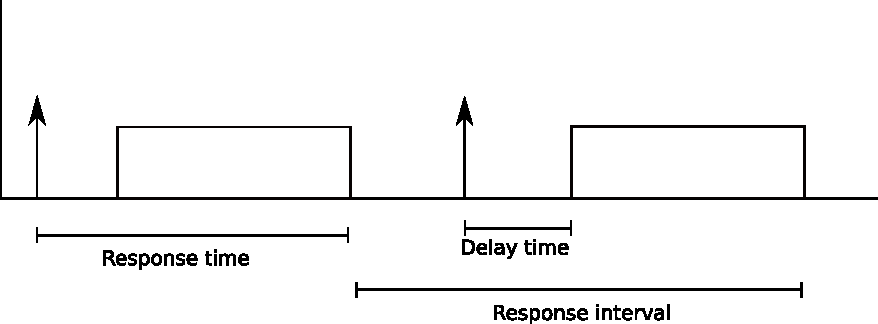
\includegraphics[scale=0.5]{metricas}
  \caption{Performance metrics}
  \label{fig:metrics}
\end{figure}

\begin{figure*}[t]
  \centering
  \subfloat[Execution costs for the trace of 'eve'.]{
    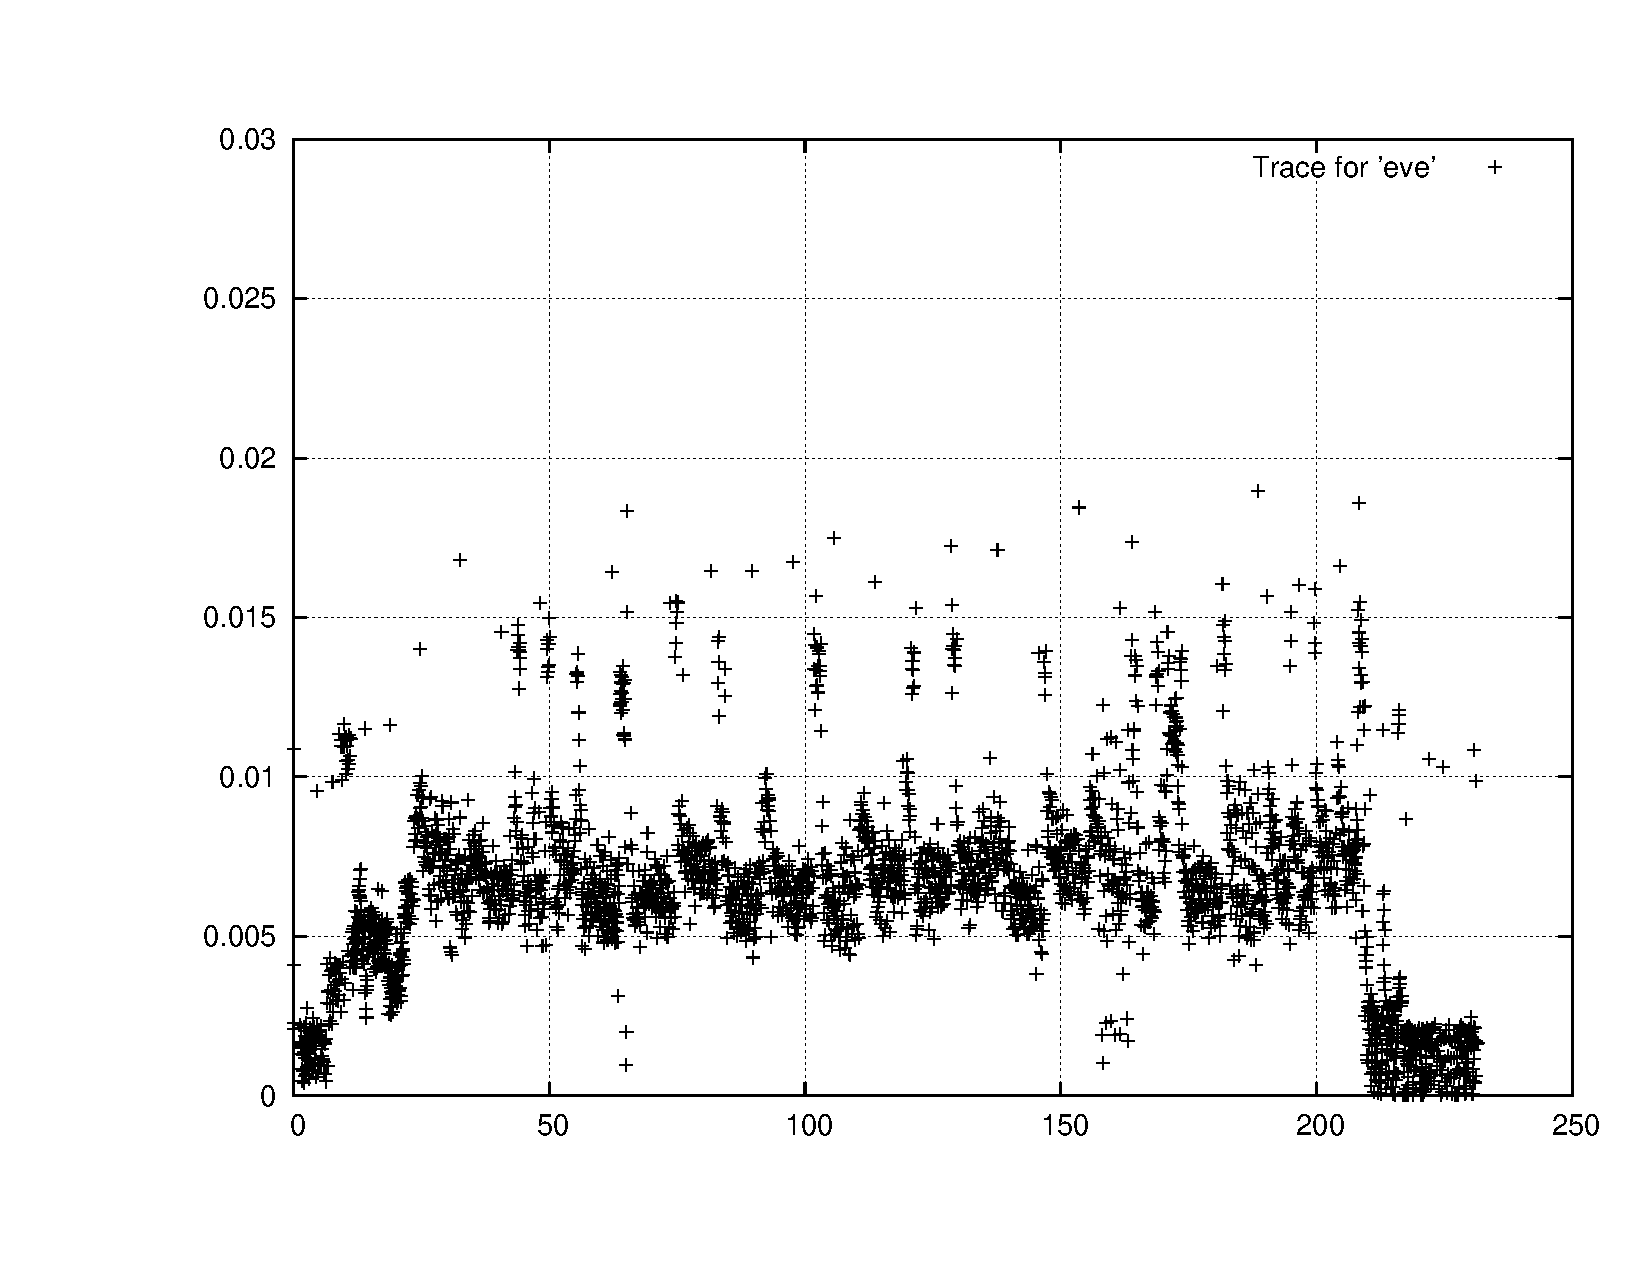
\includegraphics[scale=0.33]{trace-eve}
    \label{fig:plot-trace-eve}
  } \subfloat[Normally distributed execution costs over time. Mean 0.6
  time units, standard deviation 0.01]{
    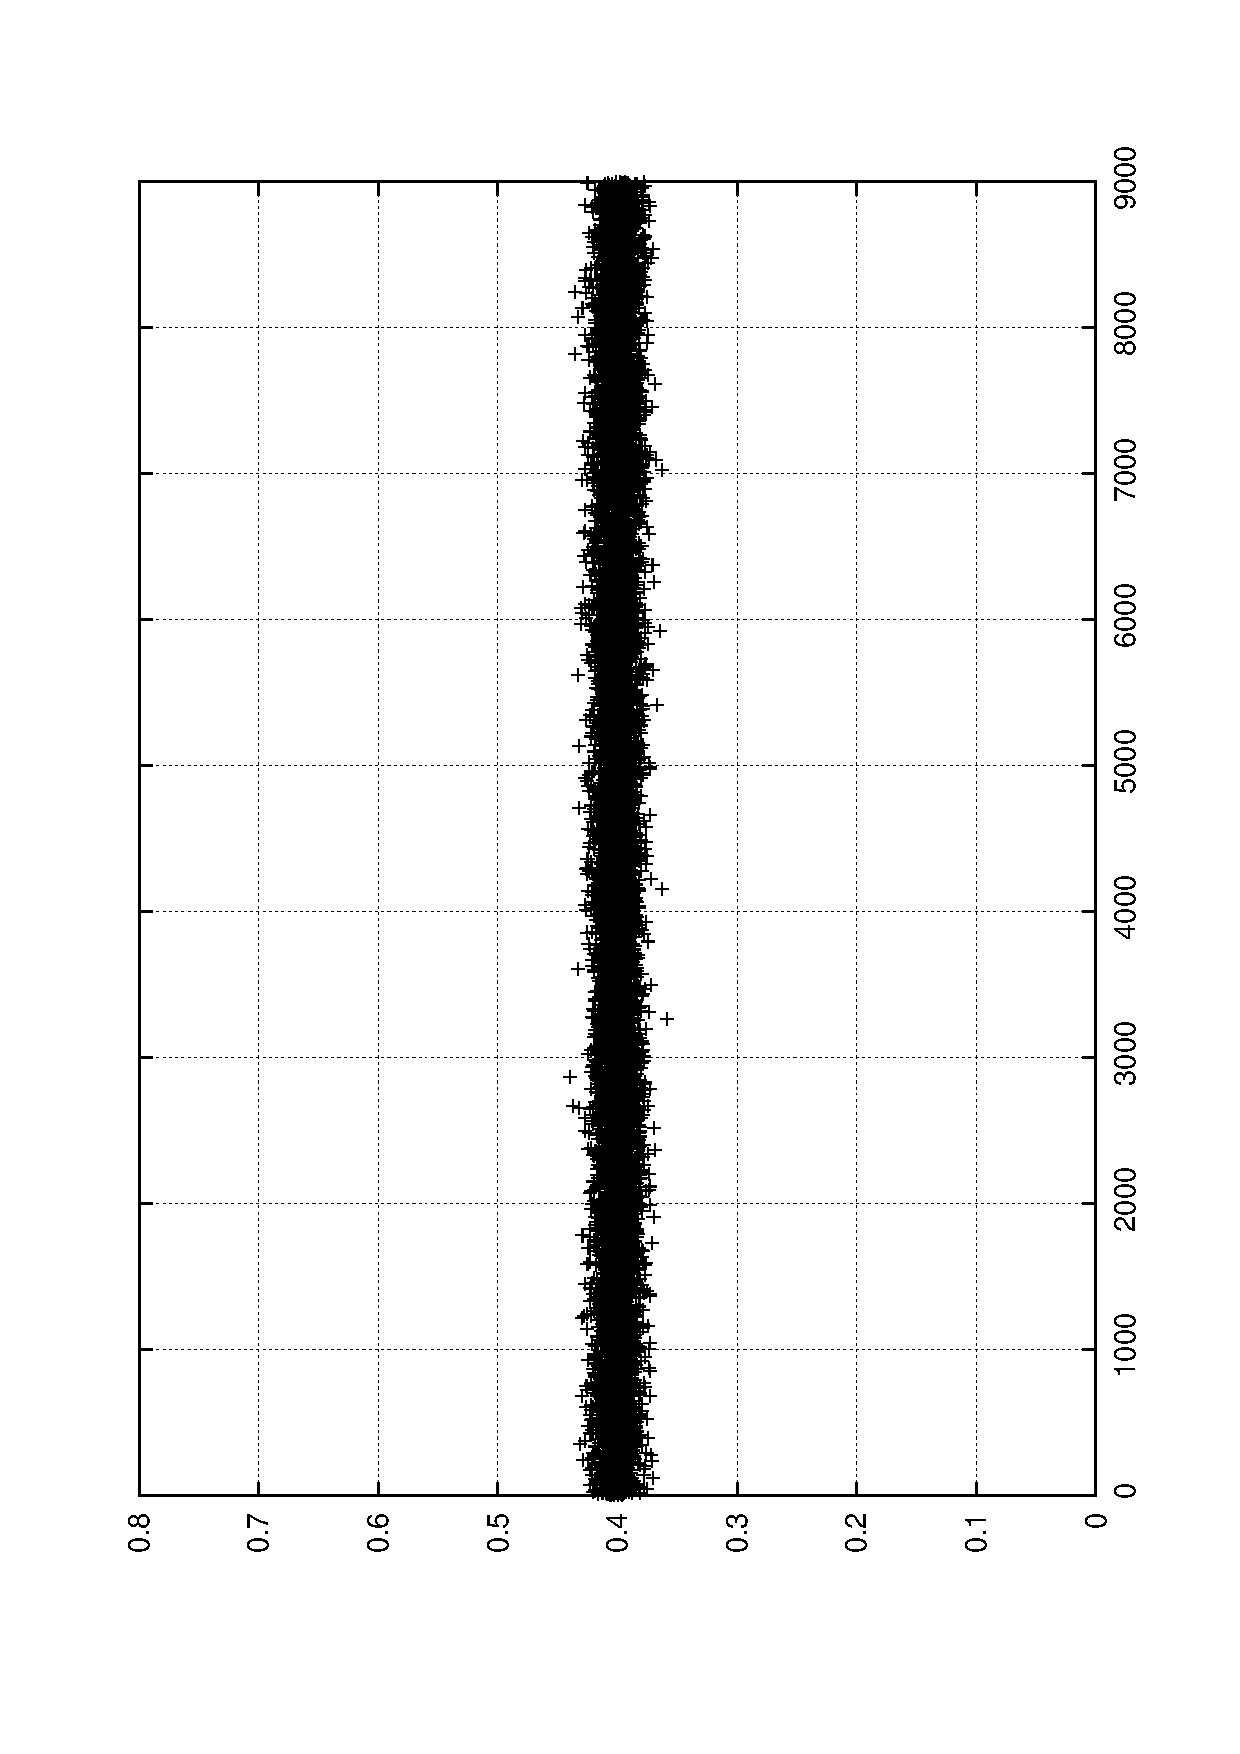
\includegraphics[scale=0.33]{trace-normal}
    \label{fig:plot-trace-normal}
  } \\
  \subfloat[Execution costs designed to simulate adaptivity. The
  standard deviation is always 0.01. The mean starts at 0.4 time
  units, goes up to 0.6 and back to 0.4.]{
    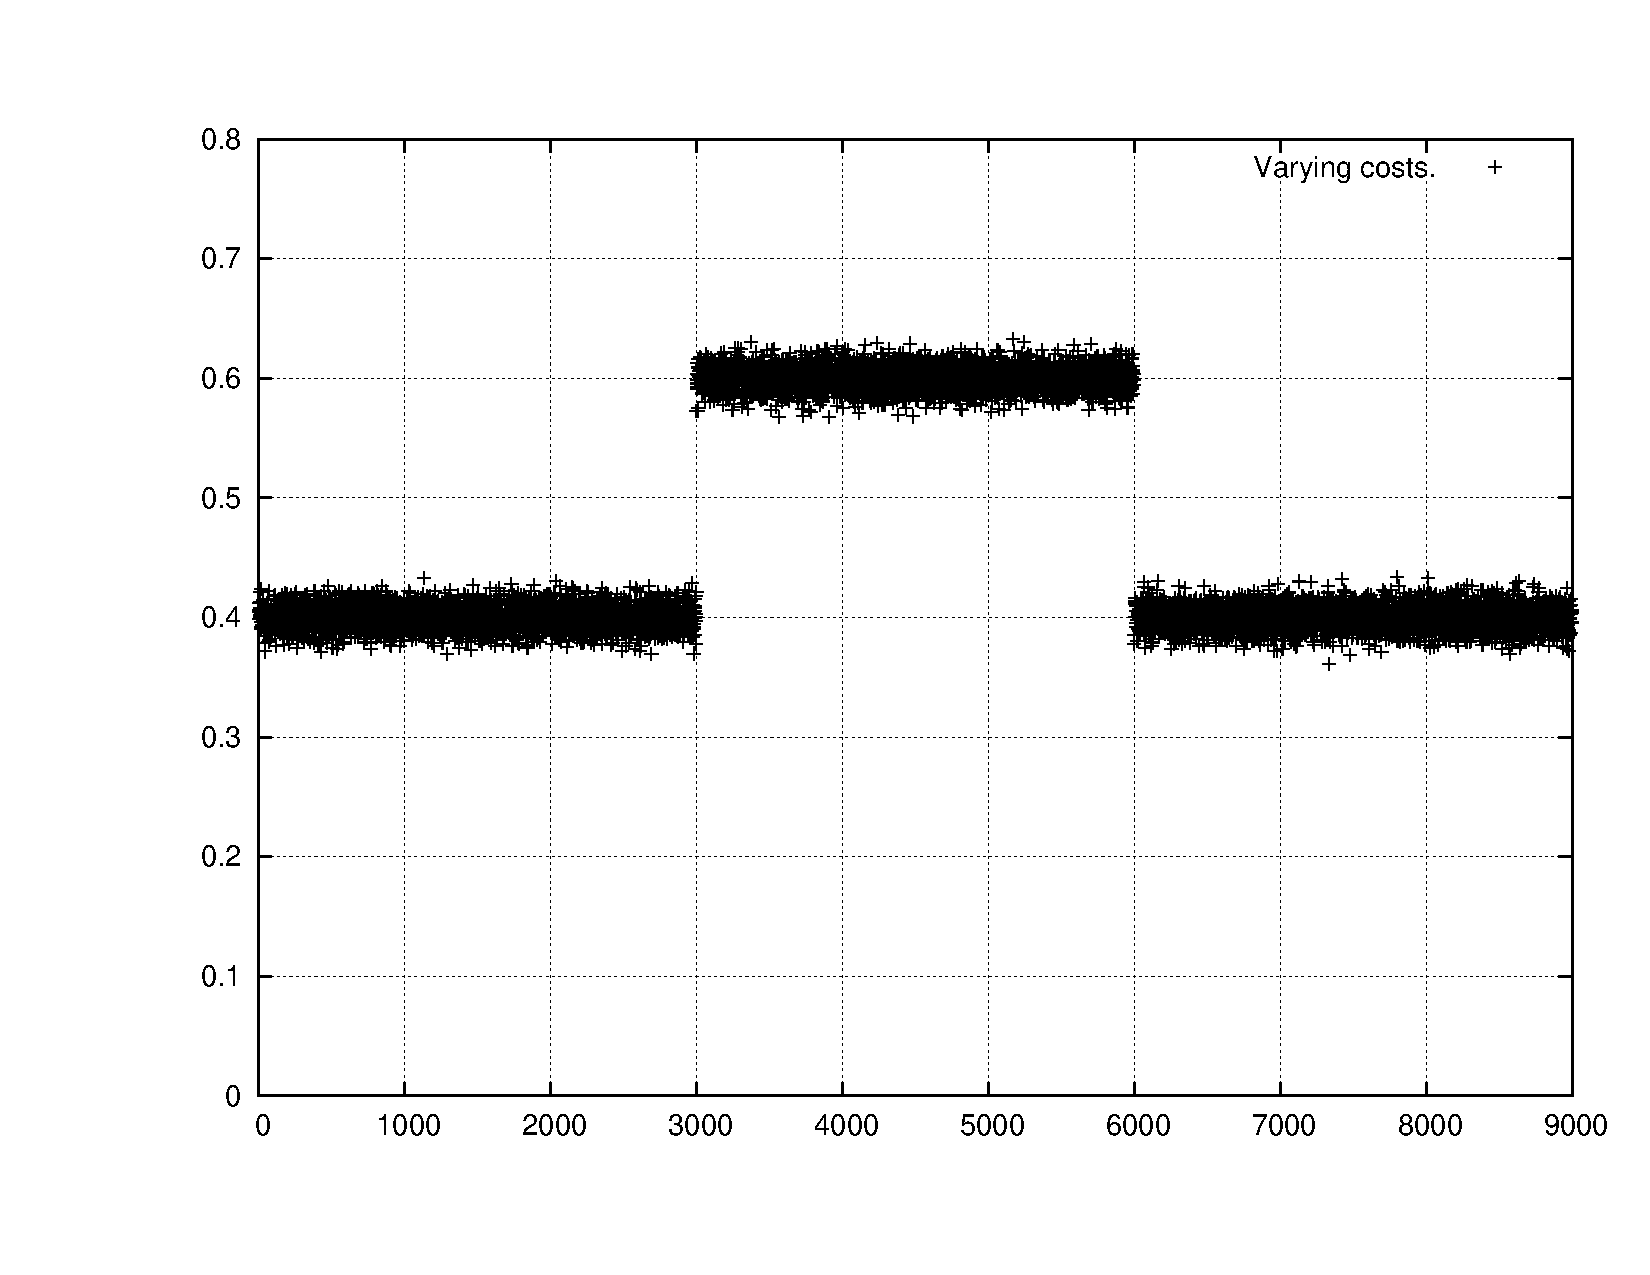
\includegraphics[scale=0.33]{trace-trifasico}
    \label{fig:plot-trace-trifasico}
  }
  \subfloat[Execution costs with low and then high variance. The mean
  is 0.5 time units and the standard deviation starts as 0.01 and goes
  up to 0.1.]{
    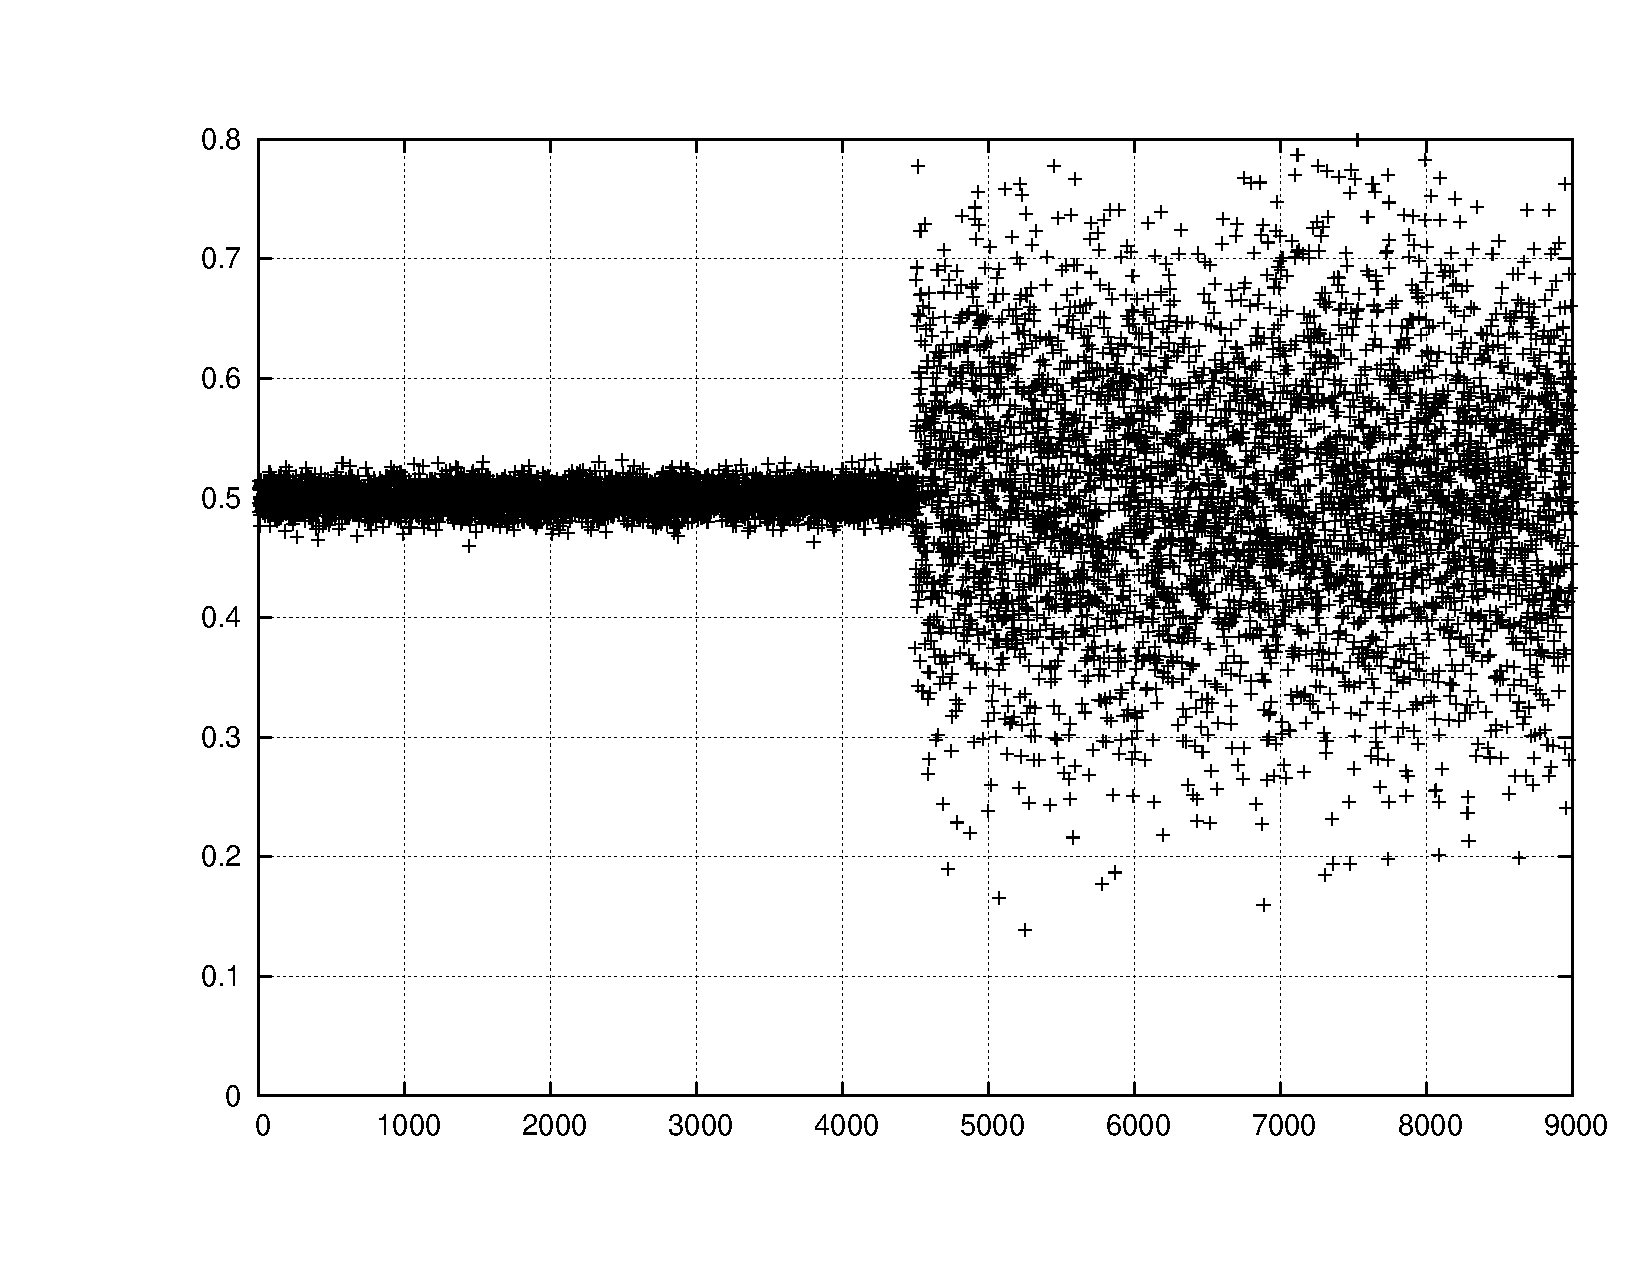
\includegraphics[scale=0.33]{trace-variance}
    \label{fig:plot-trace-variance}
  }
  \caption{Execution cost models used in our simulations.}
  \label{fig:ex-costs}
\end{figure*}


\Section{Simulation Results}
\label{sec:simulation-results}

Not all variables mentioned in section \ref{sec:controled-variables}
actually highlight any differences in performance between hard and
soft reservation.

\SubSection{Discarding expired tasks}
\label{sec:disc-expir-tasks}

We found that not discarding expired tasks makes soft and hard
reservation completely equivalent. This is easily seen from the fact
that, given the same total execution costs $t$ in a task set, both
hard and soft reservation servers with period $T_i$ and capacity $Q_i$
can only finish the task set in at least
\[ \left\lfloor\frac{t}{Q_i}\right\rfloor T_i\]
time units. The only possible difference is that a soft reservation
server might spend this budget before a hard reservation server can,
but we found that this only happens in severely underdimensioned
systems. Also, under no circumstances a hard reservation server
outperformed a soft reservation server when expired tasks were not
discarded. However, as we feel that most soft real-time systems do
discard expired tasks we believe this is unrepresentative. All other
results reported in this paper are with servers that do discard
expired tasks.

\SubSection{System load}
\label{sec:system-load}

When the system is always perfectly dimensioned or overloaded (there
is no system idle time) both reservation schemes are equivalent. This
is so because the soft server can only postpone its deadline to get
extra budget when there is free system time. This suggests that in
systems that are expected to be overloaded or in systems where all
tasks must be run until completion there is no need to worry about
using either soft or hard reservation. 

\SubSection{Server load}
\label{sec:server-load}

Another irrelevant scenario is when the server load is low enough that
there is always free budget upon completing a task. In these
situations both hard and soft reservation mechanisms are equivalent,
as there is no budget exaustion and therefore no need to postpone
deadlines.

Summarizing, the scenarios that show any difference between hard and
soft reservation happen when
\begin{itemize}
\item tasks that have overrun their deadlines are discarded,
\item there is idle time in the system,
\item but the soft real-time server is overloaded.
\end{itemize}
This leaves room for wiggling the variance of execution costs and
specific characteristics of the the task set over time.

\SubSection{Individual simulation results}
\label{sec:indiv-simul-results}

To verify the interesting cases, we performed some experiments with
synthetic normally-distributed execution costs. All data sets used in
this paper are shown in figure \ref{fig:ex-costs}.

\begin{figure*}[t]
  \centering
  \subfloat[Soft reservation.]{
    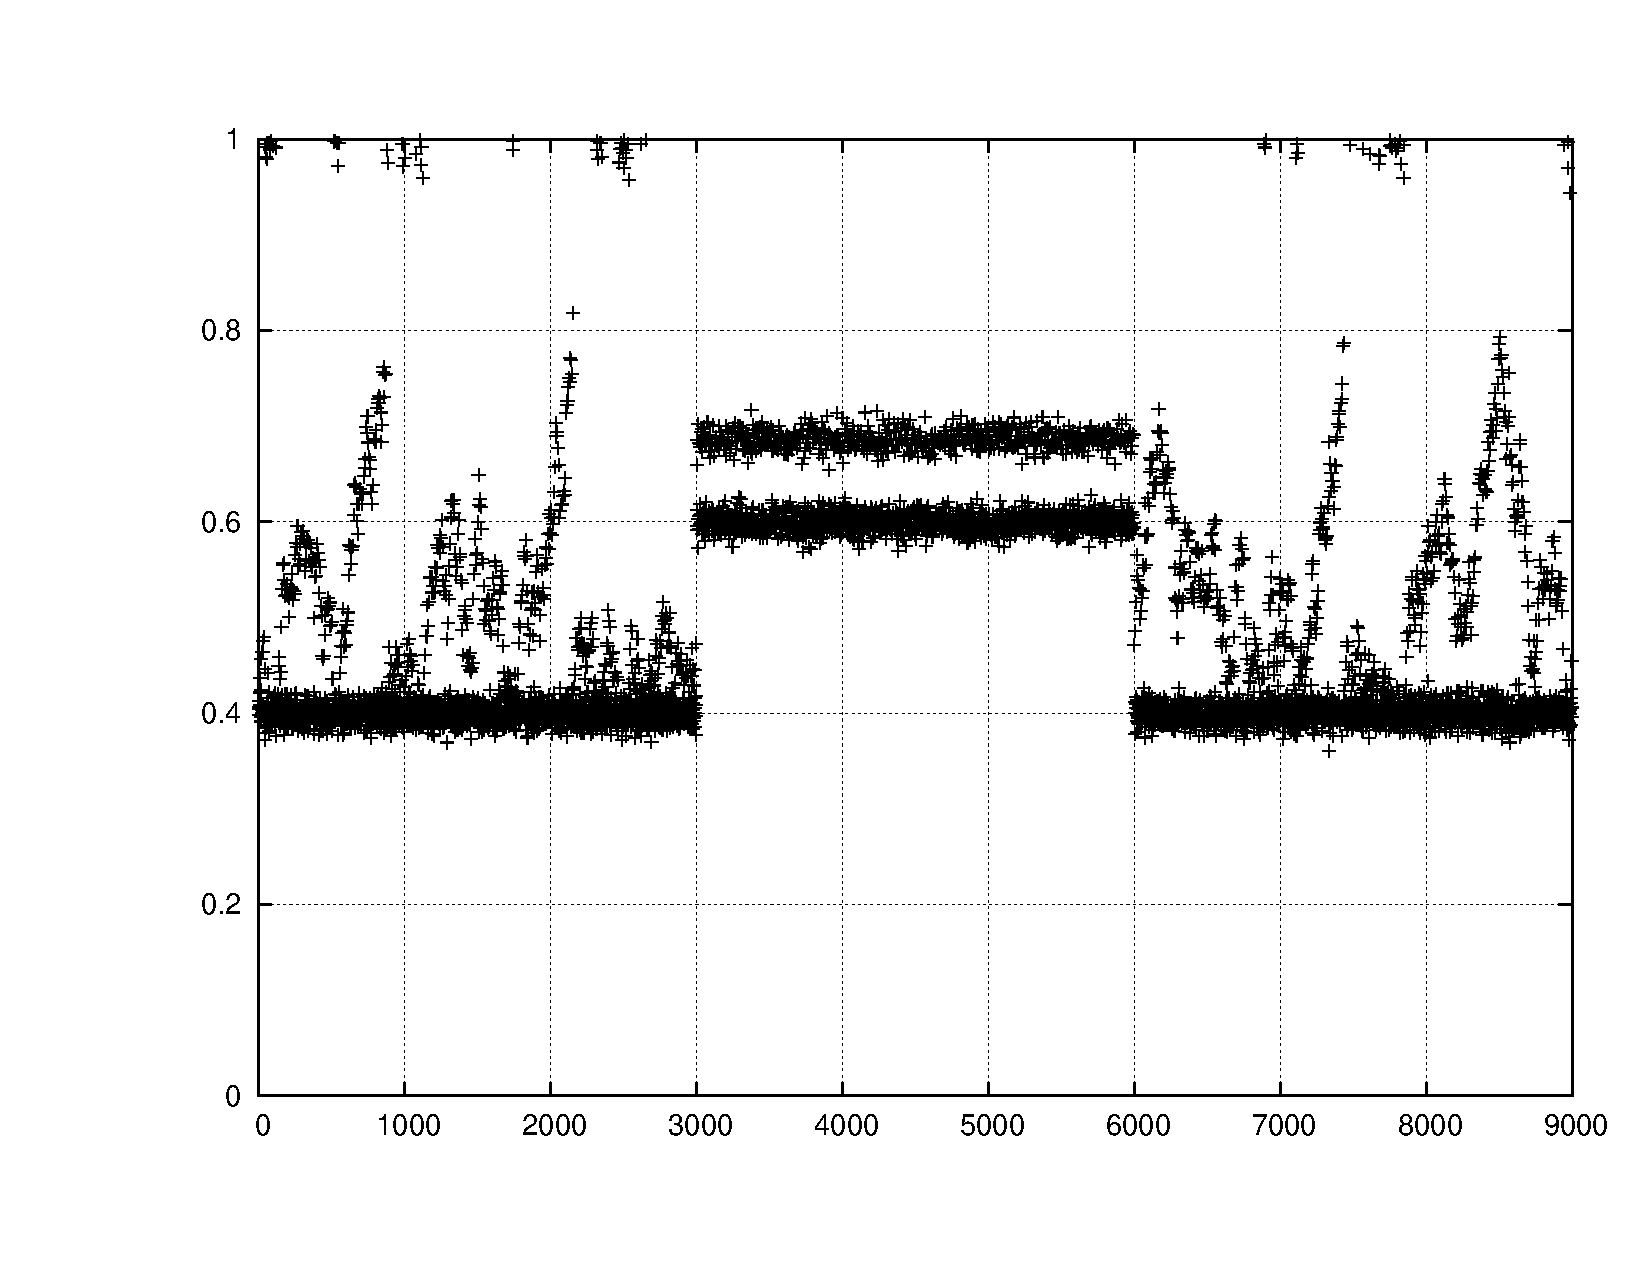
\includegraphics[scale=0.33]{trifasico-1}
    \label{fig:soft-trifasico}
  }
  \subfloat[Hard reservation.]{
    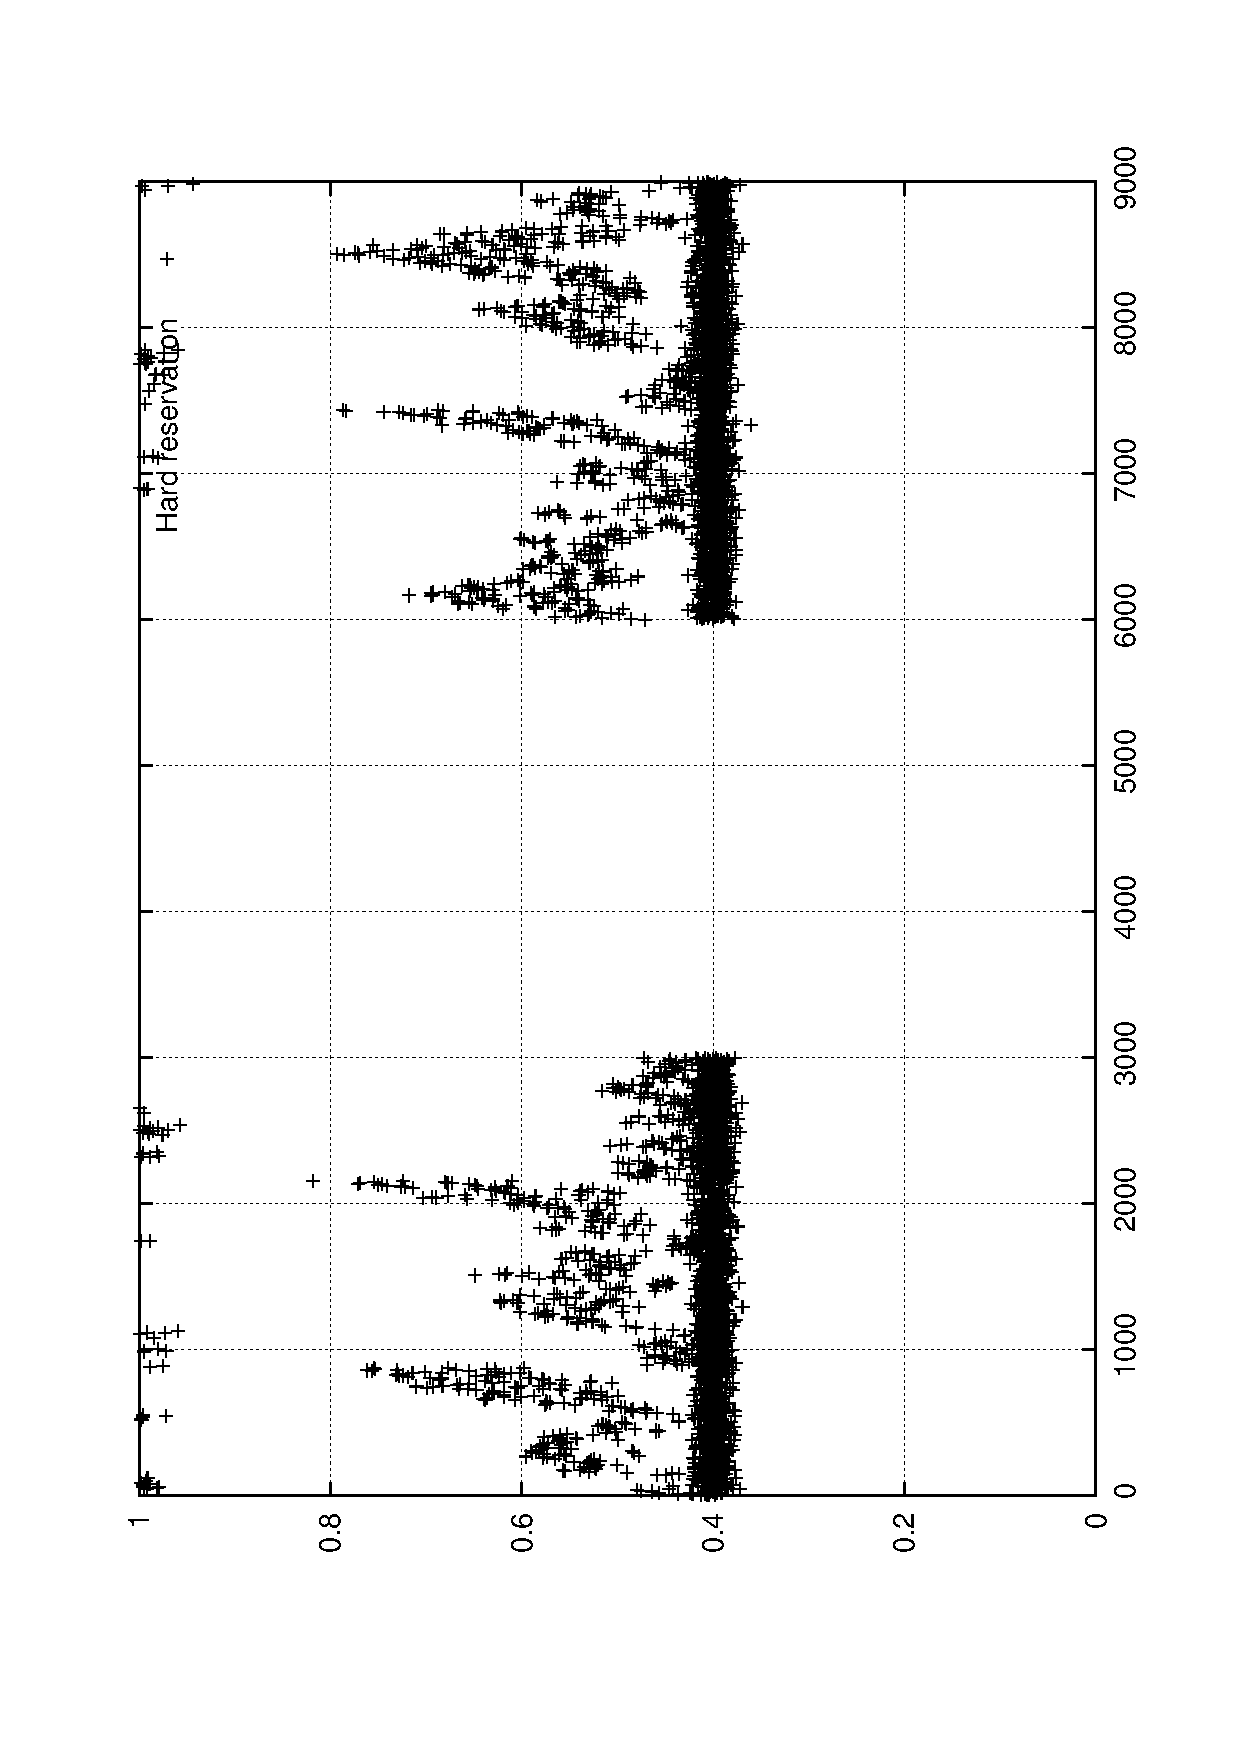
\includegraphics[scale=0.33]{trifasico-2}
    \label{fig:hard-trifasico}
  }
  \caption{Response times for the costs in figure
    \ref{fig:plot-trace-trifasico}.}
  \label{fig:trifasico}
\end{figure*}

An interesting situation happens if the real-time system runs some
adaptation mechanism, such as the one described in
\cite{abeni.ea05:qos}. Since specific adaptation mechanisms are out of
the scope of this paper, we assumed a simplistic model. In this
experiment, the task set first starts with a correctly dimensioned
server, until a certain point in time in which the mean costs for the
tasks rise suddenly. After a while, the costs return to normal. If, as
is sometimes suggested, soft reservation makes for slow adaptiveness
in these situations (by, for example, postponing the deadline too far
into the future during the high load period), a soft reservation
server running the task costs in figure \ref{fig:plot-trace-trifasico}
would be outperformed by a hard reservation server. However, as can be
seen in figure \ref{fig:trifasico}, in the heavily loaded part only
the soft reservation server can finish tasks that need more than the
server budget. As expected, when the load comes back down there is no
extra cost for the soft reservation server, and its response times are
equivalent to the hard reservation ones. This clearly shows that in
variable environments a soft reservation scheme is better than a hard
one.

\begin{figure*}[t]
  \centering
  \subfloat[Soft reservation.]{
    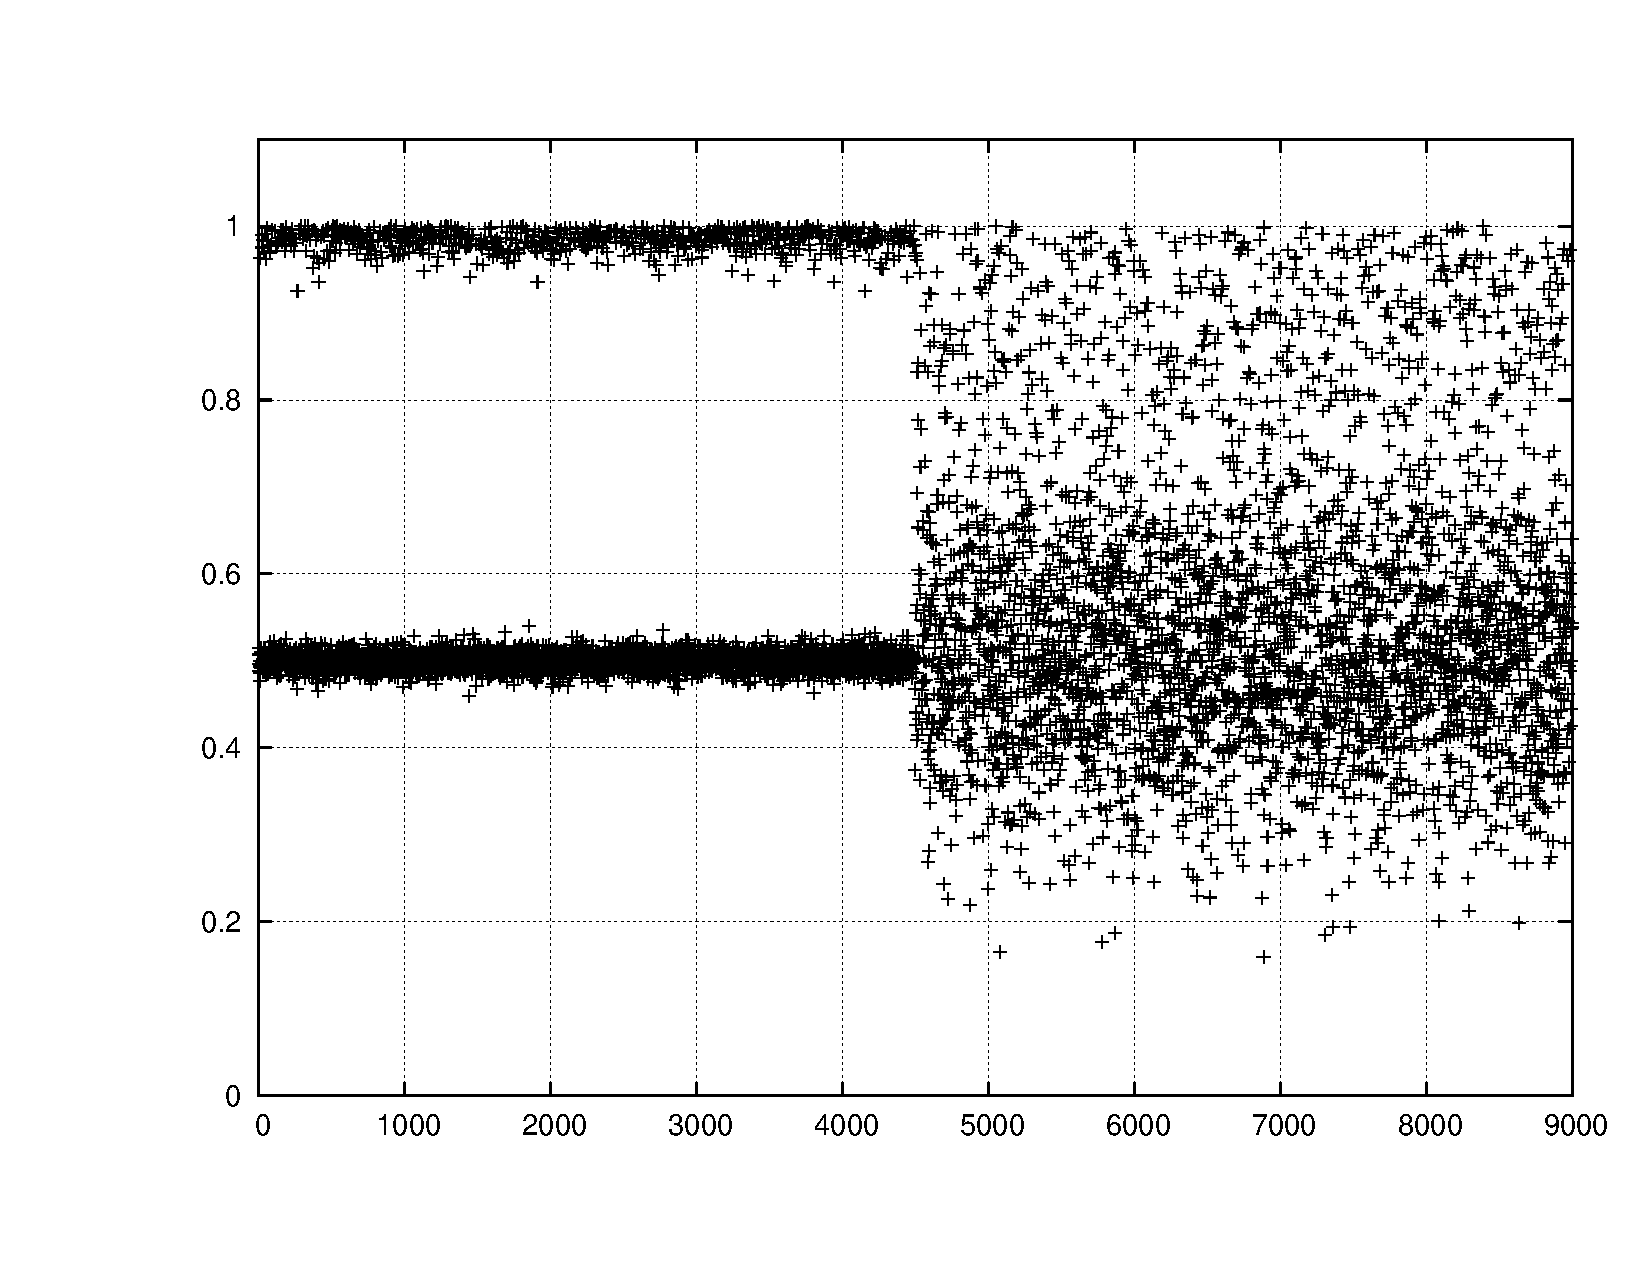
\includegraphics[scale=0.33]{variance-1}
    \label{fig:soft-variance}
  }
  \subfloat[Hard reservation.]{
    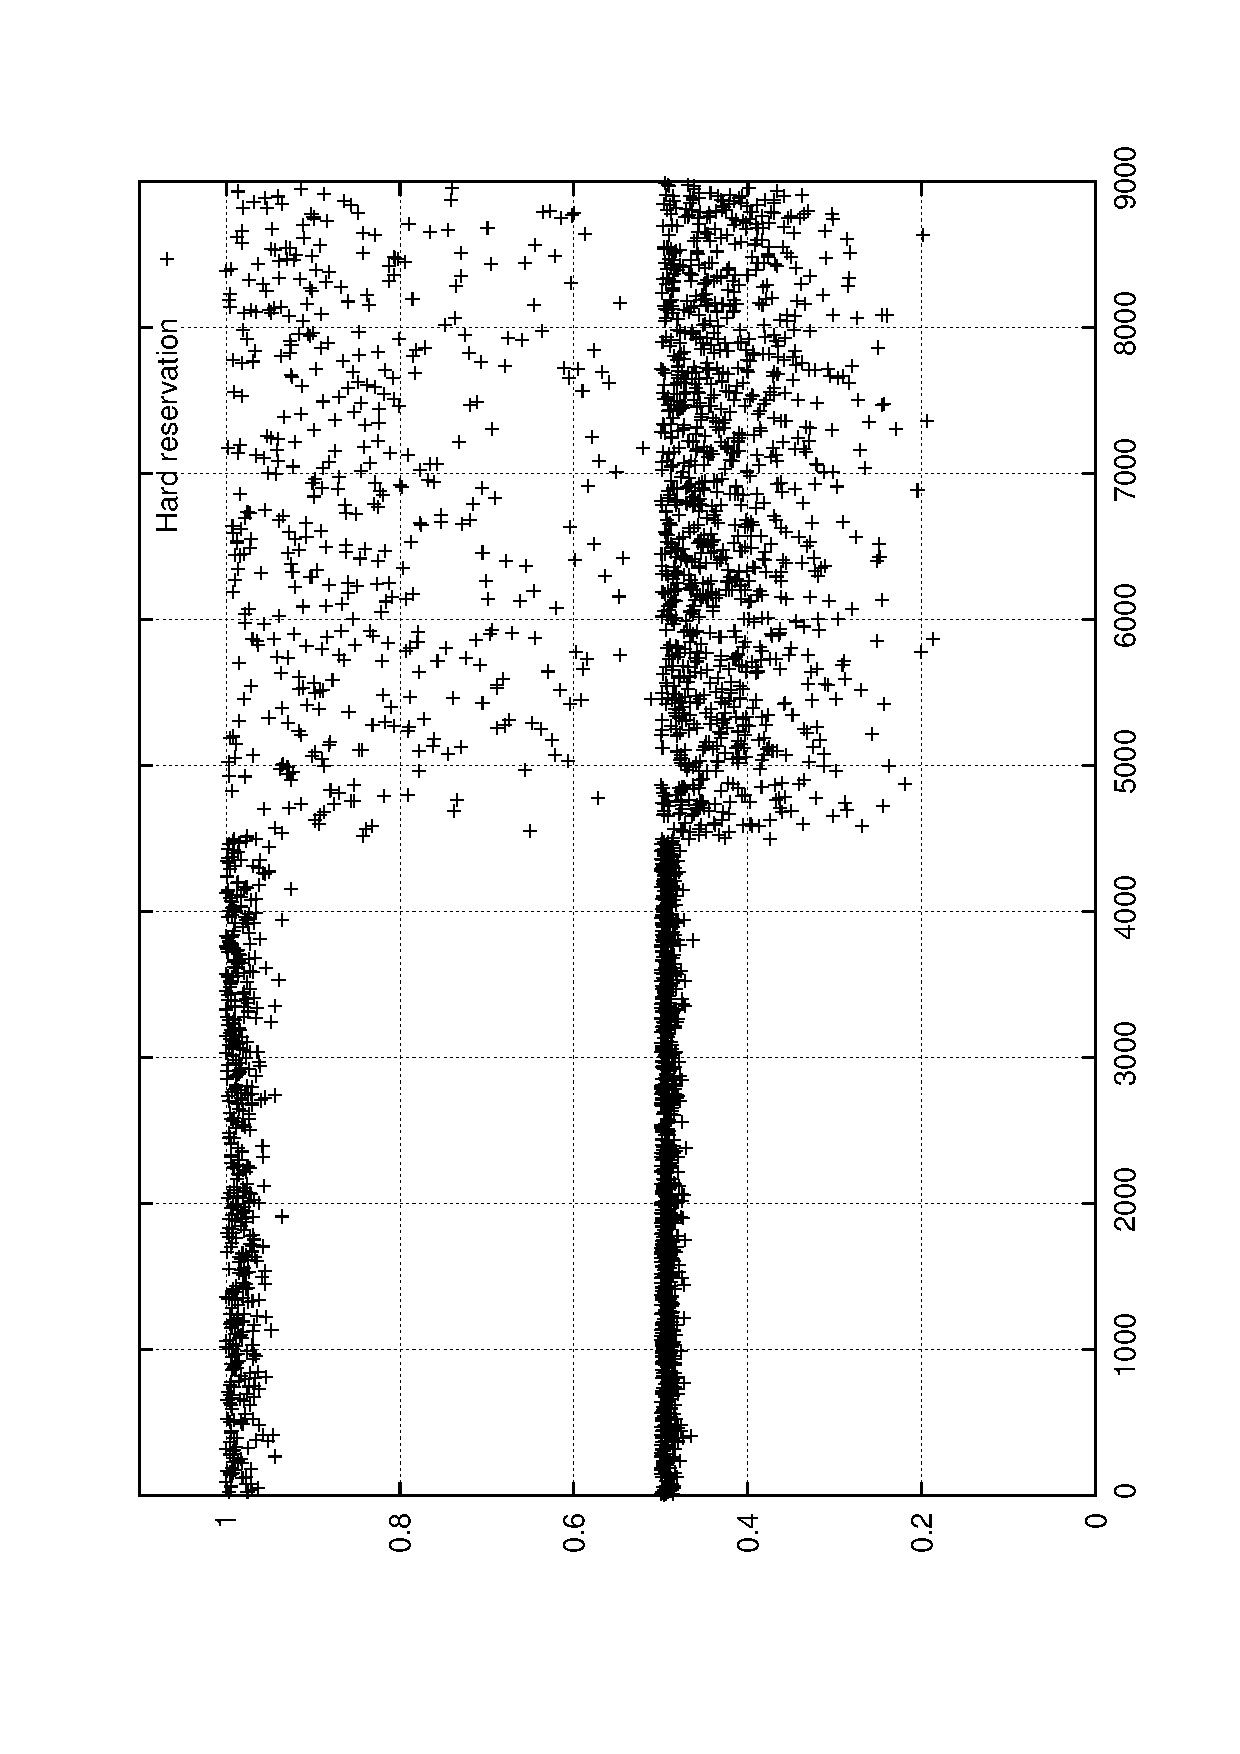
\includegraphics[scale=0.33]{variance-2}
    \label{fig:hard-variance}
  }
  \caption{Response times for the high variance case.}
  \label{fig:variance}
\end{figure*}

Another possible situation in which a soft reservation server might
have its responsivity compromised is when dealing with tasks having a
high variance in its execution costs, as in figure
\ref{fig:plot-trace-variance}. This might happen because to serve
tasks with unexpectedly high costs, a soft reservation server might
need to postpone its deadline too much, while a hard reservation
server would be more prudent and instead discard these costly
outliers, being more performant in the remaining time. In this
experiment the hard reservation server lost 59.39\% of the deadlines,
while the soft reservation only lost 5.19\%. Figure \ref{fig:variance}
shows the response times for this experiment.

\begin{figure*}[t]
  \centering
  \subfloat[Soft reservation.]{
    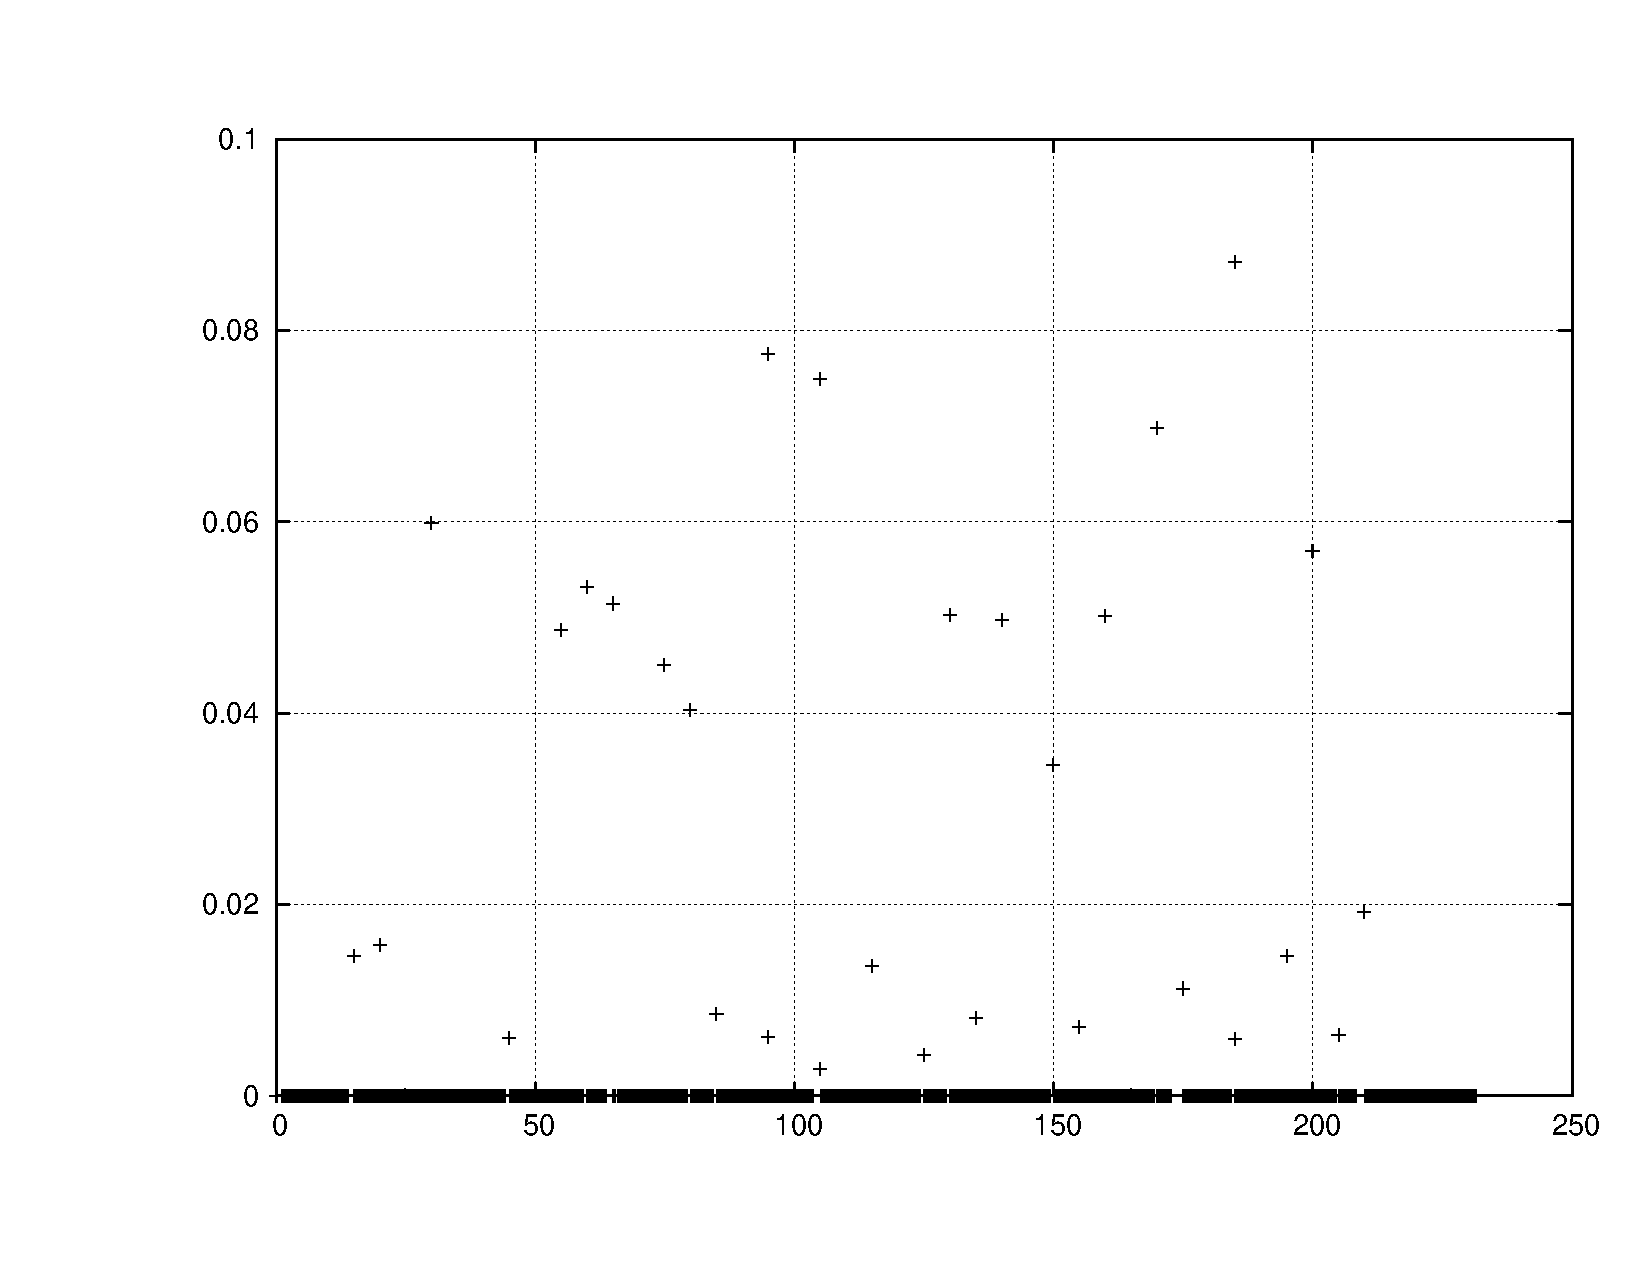
\includegraphics[scale=0.33]{eve-1}
    \label{fig:soft-eve}
  }
  \subfloat[Hard reservation.]{
    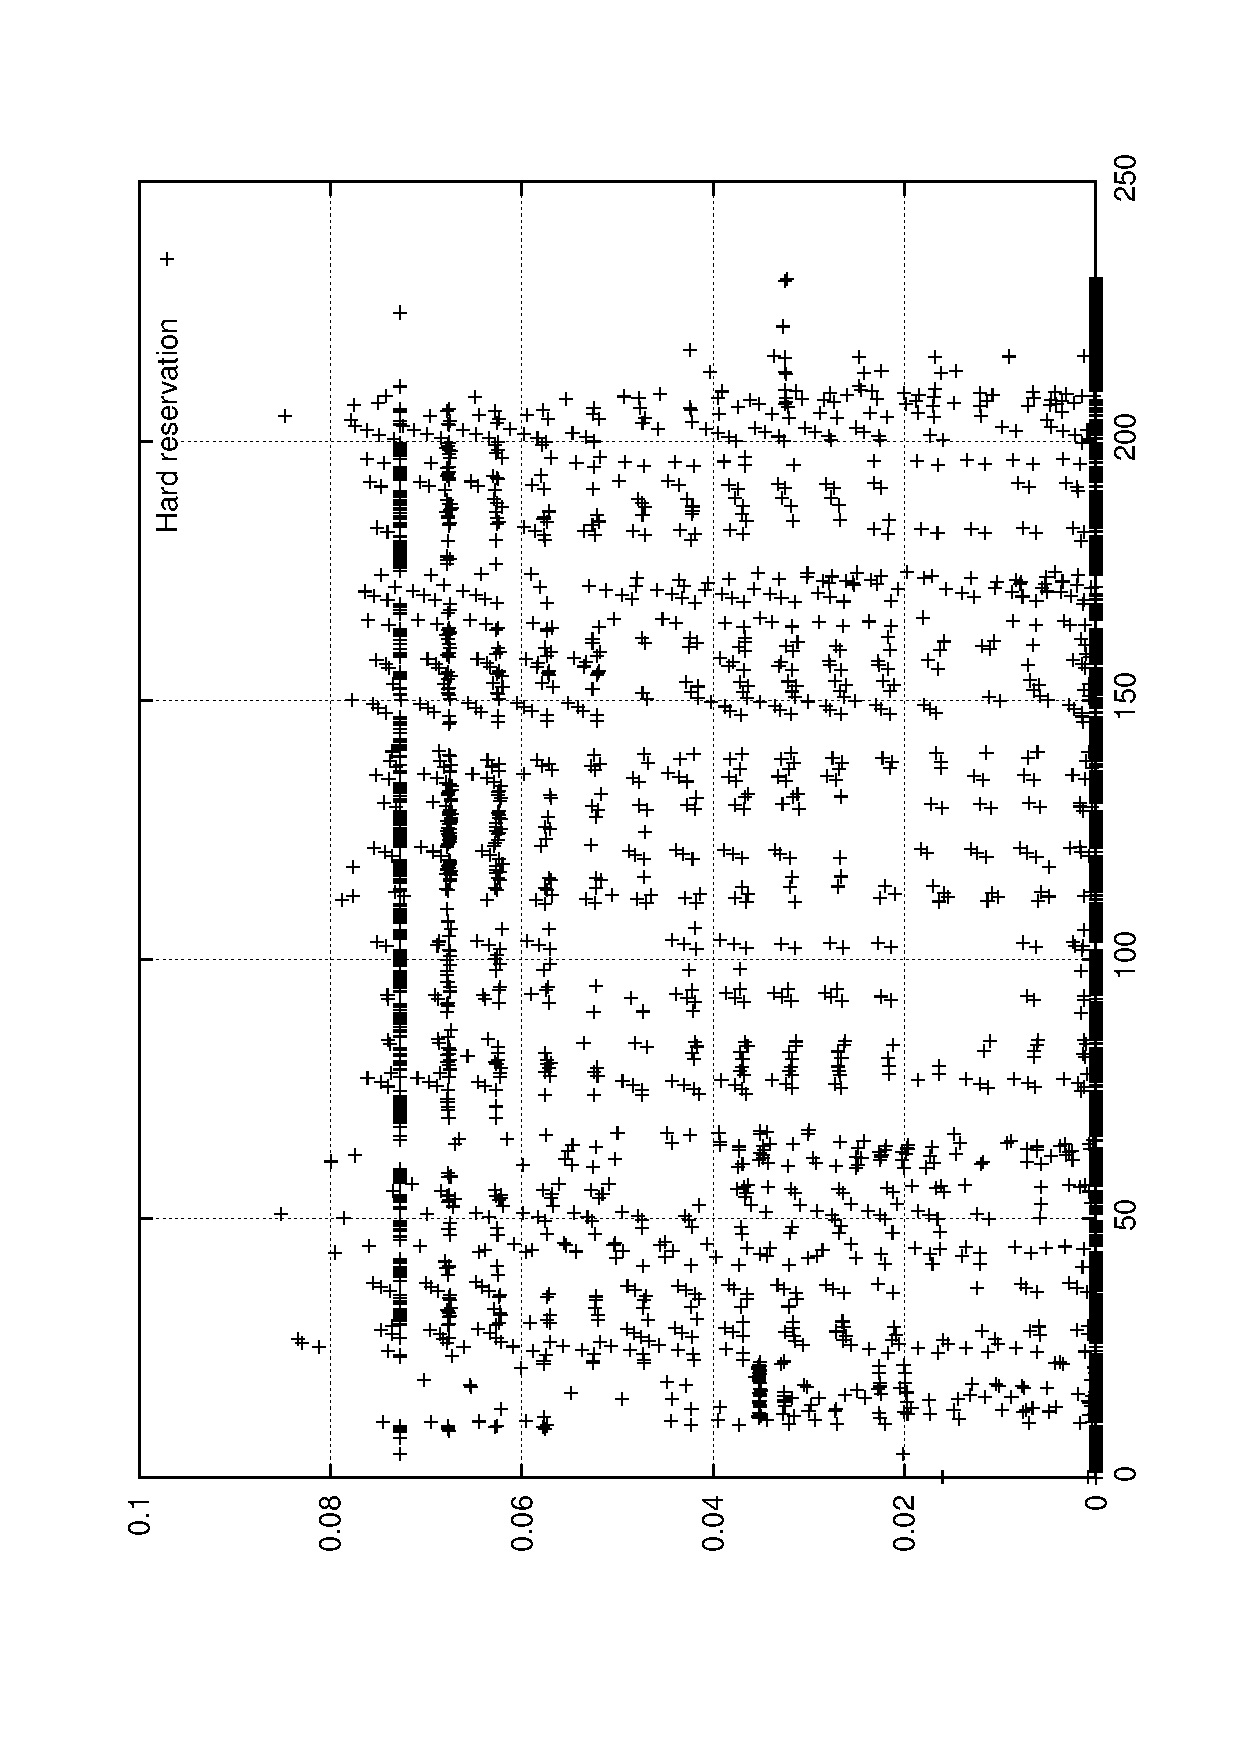
\includegraphics[scale=0.33]{eve-2}
    \label{fig:hard-eve}
  }
  \caption{Delay times for the movie trace.}
  \label{fig:eve}
\end{figure*}

Another very important test case is whether, in non-synthetic tasks,
the performance characteristics we observed are reproduced. In this
experiment, we ran both a soft reservation server and a hard
reservation server on the task set shown in figure
\ref{fig:plot-trace-eve}, a trace from decoding a high-definition
movie. Both servers had their periods set to the mean period of the
data set and their capacities were the mean costs. In the background a
hard real-time task runs consuming the remaining processor
bandwidth. As can be easily seen in figure \ref{fig:eve}, the delay
time for the hard reservation server is always higher than for the
soft reservation server. Also, the soft reservation server only lost
0.1\% of the dealines, while the hard reservation server lost
24.54\%. This result seems, at first, counter-intuitive, since the
soft reservation server, by delaying its deadline whenever the
execution costs are too high, can have an arbitrarily low priority. On
the other hand, the same task will take more overall time to be served
with a hard reservation server, since it will have to wait for
capacity replenishment before continuing execution.


\Section{Conclusion}
\label{sec:conclusion}

As can be seen in figures \ref{fig:trifasico}, \ref{fig:variance}, and
\ref{fig:eve}, soft reservation usually outperforms hard reservation,
having a smaller average response time as well as a smaller worst-case
response time, a shorter delay between task arrival and start of
execution, and a more uniform interval between successive task
terminations and misses less deadlined. 

\bibliographystyle{latex8}
\bibliography{bib}
\end{document}

\Section{Analytical characteristics}
\label{sec:analyt-char}

In \cite{buttazzo05:soft}, hard reservation is introduced as a way of
proving schedulability of a given task set using a CBS server with a
hard reservation rule. It is done o by means of the following theorems:

\begin{theorem}
  Given a CBS server with the hard reservation rule, and with
  parameters $(Q,P)$, if $k =
  \left\lceil\frac{t-(P-Q)}{P}\right\rceil$, the partition with the
  maximum delay that it can generate has the following least supply
  function $S^*(t)$:
  \[ S^*(t) = \left\{ \begin{array}{ll}
      0 & \text{if}\ t \in [0,P-Q] \\
      (k-1)Q & \text{if}\ t \in (kP - Q, (k+1)P-2Q) \\
      t-(k+1)(P-Q) & \text{otherwise.}
    \end{array}\right.
  \]
\end{theorem}

\begin{theorem}
  Let $A$ be set of periodic or sporadic tasks
  $\{\tau_1,\ldots,\tau_n\}$, with $\tau_i = (C_i,T_i,D_i)$, where
  $C_i$ is the worst-case computation time, $T_i$ is the task period
  and $D_i$ is the relative deadline. This task set is schedulable by
  EDF scheduling algorithm on a resource partition with least supply
  function $S^*(t)$ if and only if:
  \[
  \forall 0 < t \leq 2H : dbf(t) \leq S^*(t)
  \]
  where $H = lcm(T_1,\ldots,T_n)$ is the hyperperiod of A and $dbf(t)$
  is the processor demand bound function, defined as
  \[
  dbf(t) = \sum_{i=1}^n
  \left(\left\lfloor\frac{t-D_i}{T_i}\right\rfloor + 1\right)C_i.
  \]
\end{theorem}

For a proof of these results, see \cite{buttazzo05:soft}.

Interestingly, these theorems can be extended to a soft reservation
framework. Intuitively, if a given task set is schedulable on a hard
cbs server, it means that if the server budget ever runs out when
executing a task from that task set, the task still has time to finish
before its deadline. Since the total computation time available for a
given server deadline is the same under both soft and hard reservation
and no tasks from the original task set are discarded, any task set
schedulable with the hard reservation rule is schedulable with the
soft reservation rule. \nota{formalizar essa prova}

